~
\newpage
\section*{Appendix}
\addcontentsline{toc}{section}{Appendix}

\subsection*{A.1\quad Appendix to Chapter 1: An Introduction to Climate Change}
\vfill 
\begin{minipage}{\textwidth}
    \captionof{figure}{Contemporary Climate Models are Highly Accurate \label{cmip6_accuracy}}
    \centering
    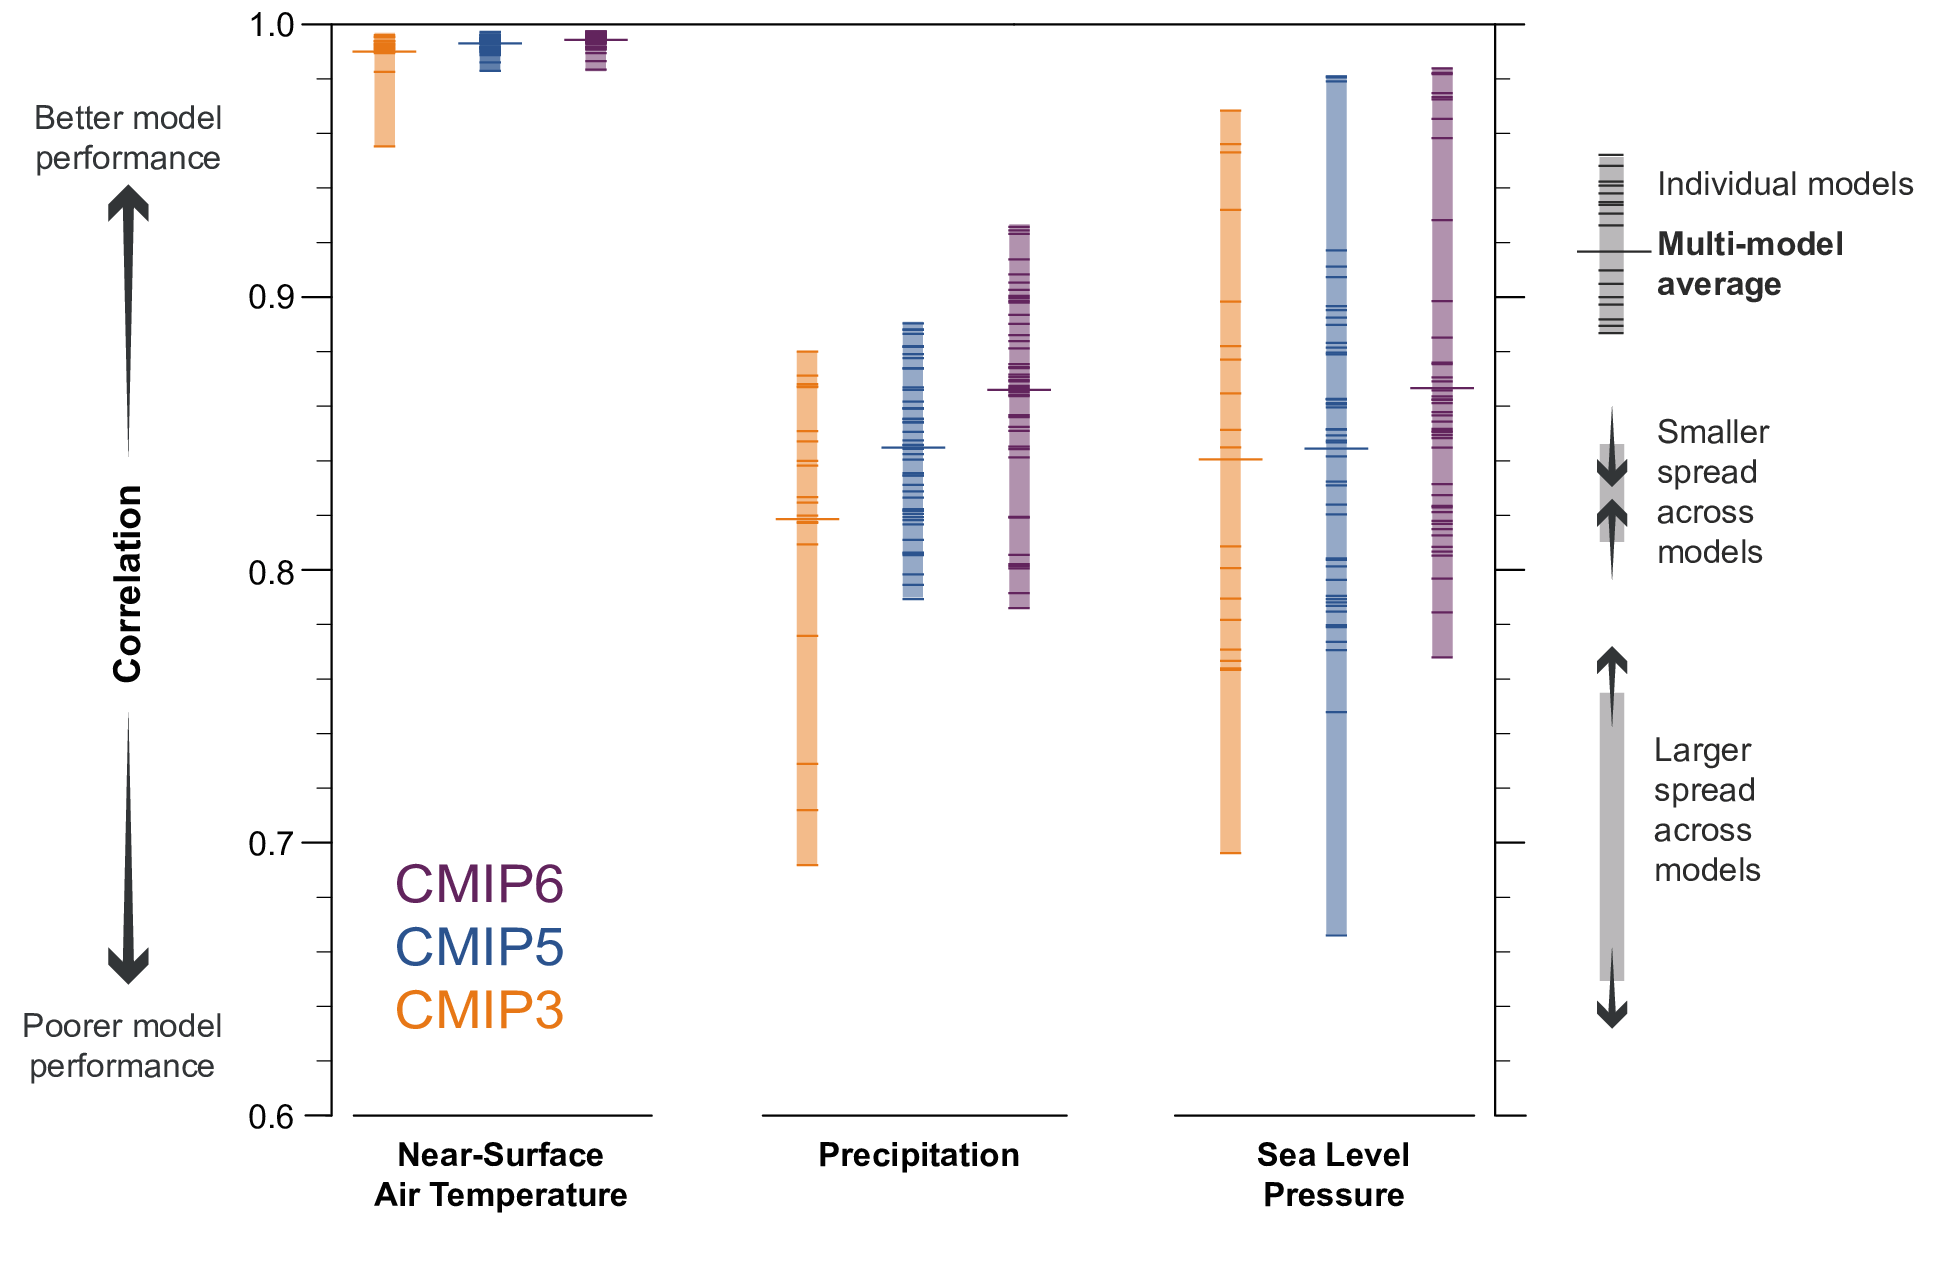
\includegraphics[width=0.7\textwidth]{figures/chapter1_figures/climate_model_accuracy.png}
    \fignote[1]{Figure from \cite{ipccAR6_model_accuracy}. The figure displays predictions for three common climate variables, near-surface air temperature, precipitation, and sea level pressure, under three different climate models. These three models are the Coupled Model Intercomparison Project Phases 3, 5, and 6. These are the three climate models used in the IPCC's fourth, fifth, and sixth assessment reports. There is no CMIP4 due to re-numbering. The vertical axis is the correlation between the model predicted outcomes the actual, observed outcomes. Clearly these models can predict near-surface air temperatures with near perfect accuracy. Other climate variables, like precipitation and sea levels rise have been more difficult to predict, but are still reasonably accurate. Climate scientists continue to learn more about the physical processes underlying climate, and consequently, these models continue to improve.
    }
\end{minipage}
\vfill

% \newpage
% \subsection*{A.2\quad Appendix to Chapter 2: Designing Climate Policy}

% \subsubsection*{The Environmental Kuznets Curve}

% The contemporary literature on the relationship between economic standard of living and environmental decay begins with Simon Kuznets, and his work related not to the environment, but inequality. \cite{kuznets1955economic} laid out a empirical relationship between economic development and inequality. Kuznets findings suggest that income inequality rises as countries move from low-income to middle-income, and income inequality falls as countries move from middle-income to high-income. Diagrammatically, this creates an inverted U-shaped path called the Kuznets Curve with GDP per capita on the horizontal axis and measures of inequality (usually the income ratio between the top quintile and bottom quintile of earners) on the vertical axis. Realizing that economic development and environmental degradation follow a similar relationship, \cite{NBERw3914} were the first to formulate the \emph{Environmental} Kuznets Curve (EKC) in an analysis of NAFTA. While the model was not the primary focus of the original paper, it later led to its own published paper, \cite{grossman1995economic} and is now a standard in environmental economics. 

% Figure \ref{EKC} displays the Environmental Kuznets Curve. The EKC hypothesizes that low-income economies will have relatively high environmental quality, as these economies may be more agrarian or pastoral. Countries often move from low-income to middle-income through industrialization, and as countries industrialize, their environmental degradation increases. Eventually though, economic development requires countries to move away from manufacturing and into higher human capital industries. When this happens, sectors dependent on high human capital (e.g., finance, engineering, education) tend to be less harsh on the environment. Past the turning point, economic development will decrease environmental degradation. 

% \begin{figure}
% \centering
% \begin{minipage}{0.48 \textwidth}
% \caption{The EKC \label{EKC}}
% \begin{tikzpicture}[scale = 0.6]
% \draw[thick, <->] (0,10) -- (0,0) -- (10,0);
% \draw[thick, color1]  [domain = 1:9] plot (\x, {8.5 - .5*(\x - 5)^2});
% \node [below right] at (7,0) {GDP/Capita};
% \node[rotate=90, above] at (0,7) {Environmental Degradation};
% \draw[dashed] (5,0) -- (5,9.5) node[right]{\footnotesize Turning Point};
% \end{tikzpicture}
% \end{minipage}
% \begin{minipage}{0.48\textwidth}
% \centering 
% \caption{Application of the  EKC}
% 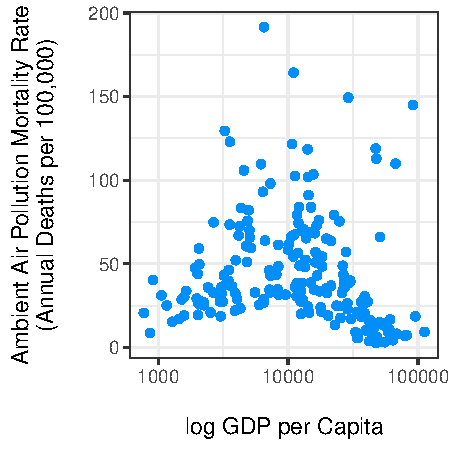
\includegraphics[width=0.9\textwidth]{figures/chapter2_figures/ekc.pdf}
% \end{minipage}
% Data from \cite{owidoutdoorairpollution} 
% %https://ourworldindata.org/outdoor-air-pollution#outdoor-air-pollution-tends-to-rise-with-industrialization-before-falling
% \end{figure}

% Despite its quick adoption in the discipline and its continued use, the EKC has largely been discredited \citep{stern2004rise}. \cite{arrow1995economic} importantly note that the usual form of the EKC does not allow for any feedback between the environment and development, implicitly assuming that pollution and other forms of environmental degradation do not hinder economic development. 

% \newpage
% \subsection*{A.3\quad Appendix to Chapter 3: Ambient Air Pollution \& Electricity Generation}



\newpage
\subsection*{A.4\quad Appendix to Chapter 4: A Model of Emissions Pricing \& Environmental Inequality}

\begin{center}
    \singlespacing
    \renewcommand{\arraystretch}{1.5}
    \captionof{table}{Overview of Notation\label{notation}}
    \small
\begin{longtable}{c L{0.55\textwidth} C{0.15\textwidth} c}
    \hline\hline 
    Variable & Description & Determined & Source\\
    \hline \\[-1.8ex]
    \multicolumn{4}{l}{\emph{Indices \& Model Environment}}\\
    \hline 
    $i$ & Power plant identifier & -- & -- \\
    $r$ & Region identifier & -- & -- \\
    $\ell$ & Transmission line identifier & -- & -- \\
    $m$ & Subregion or community identifier & -- & --\\ 
    $N$ & The number of power plants & Exogenous & (1) \\
    $\mathcal{N}$ & Set of all power plants; $\mathcal{N} = \{1, \ldots, N\}$ & Exogenous & (1) \\
    $\mathcal{N}_r$ & Set of all power plants in region $r$ & Exogenous &  (1) \\
    $R$ & The number of regions & Exogenous &  (1) \\
    $\mathcal{L}$ & Set of all transmission lines & Exogenous &  (5) \\
    $M$ & Number of subregions or communities & Exogenous &  (3), (4)\\
    $T$ & Final period of the generation phase & Exogenous &  Chosen\\
    \\[-1.8ex]
    \multicolumn{4}{l}{\emph{Investment Phase}}\\
    \hline 
    $\mathcal{J}$ & Set of all investment options & Exogenous & Chosen\\
    $j_i$ & Power plant $i$'s investment decision; $j_i \in \mathcal{J}$ & Endogenous & -- \\
    $j$ & Investment profile, $j = (j_1, j_2, \ldots, j_N)$ & Endogenous & -- \\
    $\rho_i^0$ & Power plant $i$'s initial heat rate (Btu/kWh) & Exogenous & (1) \\
    $\rho_i$ & Power plant $i$'s heat rate (Btu/kwh) & Endogenous & -- \\
    $\tilde{\delta}$ & Heat rate depreciation rate from the investment phase to the generation phase; $\tilde{\delta} \in (0, 1)$ & Exogenous & (10) \\
    $v_i$ & Power plant $i$'s stochastic investment cost shock; $v_i > 0$ for all $i \in \mathcal{N}$ & Exogenous & Chosen \\
    $\gamma$ & Constant scalar in the investment cost function; $\gamma > 0$ & Exogenous & (12) \\
    $\alpha$ & Scale parameter in the investment cost function; $\alpha > 0$ & Exogenous & (12) \\
    $\Gamma (j_i, v_i)$ & Investment costs for power plant $i$; a function of power plant $i$'s investment choice $j_i$ and $i$' stochastic investment cost shock $v_i$ & Endogenous & -- \\
    $\Gamma (j \mid v)$ & Total investment costs for all power plants; a function of the investment profile $j$ given a vector of all power plants' stochastic investment cost shocks $v$ & Endogenous & -- \\
    $Q_t^e$ & $R$-dimensional vector of expected quantities demanded of electricity at time $t$ for each region (kWh) & Exogenous & (2)\\
    \\[-1.8ex]
    \multicolumn{4}{l}{\emph{Generation Phase}}\\
    \hline 
    $a_{it}$ & Operating decision of power plant $i$ in period $t$; $a_{it} \in \{0, 1, \ldots, R\}$ where $a_{it} = r$ indicates that power plant $i$ operates in period $t$ to sell its generation in region $r$ and $a_{it} = 0$ indicates that power plant $i$ does not operate in period $t$ & Endogenous & -- \\
    $a_t$ & Profile of operating decisions in period $t$; $a_t = (a_{1t}, a_{2t}, \ldots, a_{Nt})$ & Endogenous & -- \\
    $\overline{q}_i$ & Power plant $i$'s nameplate capacity (kW); the maximum rated generation of power plant $i$ in an hour & Exogenous & (1) \\
    $q_{itr}$ & Power plant $i$'s generation to be sold in region $r$'s wholesale electricity market at time $t$ (kWh) & Endogenous & -- \\
    $f_i$ & The primary fuel type of power plant $i$; $f_i \in \{\text{Coal}, \text{Natural Gas}, \text{Oil}\}$ & Exogenous &  (1) \\
    $u_{f_i}$ & Unit cost of power plant $i$'s fuel $f_i$ (\$/Btu) & Exogenous & (6), (7), (8)\\
    $e_{f_i}$ & Greenhouse gas emissions intensity of power plant $i$'s fuel $f_i$ (tonnes CO$_2$e/Btu) & Exogenous & (1)\\
    $\tau_r$ & Greenhouse gas emissions tax in region $r$ (\$/tonnes CO$_2$e) & Exogenous & (9) \\
    $P_{tr}$ & Price of electricity in region $r$'s wholesale market at time $t$ & Endogenous & -- \\
    $Q_{tr}$ & Quantity of electricity demanded in region $r$'s wholesale market at time $t$ & Exogenous &  (2) \\
    $C(a_t\mid j)$ & Total cost of generation in period $t$; a function of the profile if operating decisions $a_t$ given the profile of investment decisions $j$ & Endogenous & -- \\
    $MC(j)$ & Marginal cost matrix, $N \times R$; a function of the investment profile (vector) $j$; element in the $i$th row and $r$th column is $mc_{ir}$ & Endogenous & -- \\
    $G(a_t)$ & Generation matrix, $N \times R$; a function of the operating decision profile (vector) $a_t$; element in the $i$th row and $r$th column is $q_{itr}$ or $\overline{q}_i \1(a_{it} = r)$ & Endogenous & --\\
    $\rho^0$ & $N$-dimensional vector of heat rates in the absence of investment; the $i$th element is $\rho_i^0(1 + \tilde{\delta})$ & Endogenous & -- \\
    $D_{\rho^0 - j}$ & Diagonalized $N\times N$ matrix corresponding with the vector $\rho^0 - j$; for elements along the diagonal, the element in the $i$th row and $i$ column is $\rho_i = \rho_i^0(1 + \tilde{\delta}) - j_i$, all elements not along the diagonal are 0 & Endogenous & -- \\
    $U$ & Unit cost matrix, $N\times R$; the element in the $i$th row and $r$th column is power plant $i$'s cost in region $r$ per Btu, $u_{f_i} + e_{f_i}\tau_r$ & Derived & -- \\
    $\overline{q}$ & $N$-dimensional vector of nameplate capacities; $\overline{q} = (\overline{q}_1, \overline{q}_2, \ldots, \overline{q}_N)$ & Derived & -- \\
    $D_{\overline{q}}$ & Diagonalized $N\times N$ matrix corresponding with the vector $\overline{q}$; for elements along the diagonal, the element in the $i$th row and $i$th column is $\overline{q}_i$, all elements not along the diagonal are 0 & Derived & -- \\
    $\1(a_t)$ & Operating decisions matrix, $N \times R$; the element in the $i$th row and $r$th column is $\1(a_{it} = r)$ & Endogenous & -- \\
    $\delta$ & Hourly discount factor, $\delta \in (0, 1)$ & Exogenous & (10)\\
    $y_{tr}$ & Net electricity exports for region $r$ at time $t$; alternatively, understood as a marginal power injection out of region $r$ at time $t$ & Endogenous & -- \\
    $PTDF_{r\ell}$ & Power transfer distribution factor on transmission line $\ell$ out of region $r$ & Exogenous & (5)\\
    $\text{Cap}_\ell$ & Maximum capacity of transmission line $\ell$ (kW) & Exogenous & (5)\\
    \\[-1.8ex]
    \multicolumn{4}{l}{\emph{The EI Gap}}\\
    \hline 
    $d$ & $M$-dimensional vector of communities' disadvantaged status; the $m$th element is 1 is $m$ is a disadvantaged community and 0 otherwise & Exogenous & (3), (4)\\
    $w$ & Local air pollutant identifier & -- & -- \\
    $e_i^w$ & Power plant $i$'s emissions intensity of air pollutant $w$ (pounds/kWh) & Exogenous & (1)\\
    $w_{it}$ & Power plant $i$'s emissions of air pollutant $w$ (lbs) & Endogenous & -- \\
    $\phi_w(w_{it}\mid i, t)$ & $M$-dimensional vector of the changes in the concentration of air pollutant $w$ across all $M$ communities resulting from $w_{it}$, the emissions of air pollutant $w$ from power plant $i$ in time $t$ & Endogenous & -- \\
    $\Phi_w^1(T)$ & Average change in the concentration of pollutant $w$ for disadvantaged communities (elements of $d$ equal to 1) after $T$ periods & Endogenous & -- \\
    $\Phi_w^0(T)$ & Average change in the concentration of pollutant $w$ for non-disadvantaged communities (elements of $d$ equal to 0) after $T$ periods & Endogenous & -- \\
    $\text{EIGap}_w(T)$ & The environmental inequality gap after $T$ periods & Endogenous & -- \\
    \hline\hline
\end{longtable}
\fignote[1]{Table summarizes the notation used in Chapter 4. In general, lowercase letters without an index are profiles/vectors, plain-text uppercase letters denote matrices or the size of a set, and uppercase letters in the \texttt{mathcal} font are sets (e.g., $\mathcal{N}$). We denote the equilibrium of any variable as the variable with an asterisk. Derived variables are those that are a deterministic function of entirely exogenous variables. The source key for exogenous variables correspond with the data sources in Table \ref{data_sources}.}
\end{center}

\newpage
\subsection*{A.5\quad Appendix to Chapter 5: Carbon Pricing \& Air Pollution Disparities in California}

\begin{center}
    \singlespacing
    \renewcommand{\arraystretch}{1.5}
    \captionof{table}{Data Sources Key\label{data_sources}}
    \small
    \begin{longtable}{c L{0.8\textwidth}}
        \hline\hline
        Source Key & Source Citation\\
        \hline \\[-3ex]
        (1) & United States Environmental Protection Agency (EPA). 2021. ``Emissions \& Generation Resource Integrated Database (eGRID), 2019" Washington, DC: Office of Atmospheric Protection, Clean Air Markets Division. Available from EPA's eGRID web site: \url{https://www.epa.gov/egrid}.\\ \\[-3ex]
        \hline \\[-3ex]
        (2) & United States Energy Information Administration (EIA). 2023. ``Hourly Electric Grid Monitor'' Region Files. Available at: \url{https://www.eia.gov/electricity/gridmonitor/dashboard/electric_overview/US48/US48}\\ \\[-3ex]
        \hline \\[-3ex]
        (3) & United States Environmental Protection Agency. 2021 version. EJScreen. Census Tract-Level US Percentiles. Retrieved: 2023-03-03. Available at: \url{https://gaftp.epa.gov/EJSCREEN/2021/} \\ \\[-3ex]
        \hline \\[-3ex]
        (4) & California Office of Environmental Health \& Hazard Assessment (OEHHA). 2022. SB 535 Disadvantaged Communities. Retrieved: 2023-03-03. Available at: \url{https://oehha.ca.gov/calenviroscreen/sb535} \\ \\[-3ex]
        \hline \\[-3ex]
        (5) & Fowlie, Meredith, Petersen, Claire, and Reguant, Mar. Data and Code for: Border Carbon Adjustments When Carbon Intensity Varies Across Producers: Evidence from California. Nashville, TN: American Economic Association [publisher], 2022. Ann Arbor, MI: Inter-university Consortium for Political and Social Research [distributor], 2021-05-13. \url{https://doi.org/10.3886/E131024V1} \\ \\[-3ex]
        \hline \\[-3ex]
        (6) & United States Energy Information Administration. 2023. Natural Gas Electric Power Price. Source key: N3045. Available at: \url{http://www.eia.gov/dnav/ng/ng_pri_sum_a_epg0_peu_dmcf_m.htm} \\ \\[-3ex]
        \hline \\[-3ex]
        (7) & United States Energy Information Administration. 2023. Coal shipments to the electric power sector: price, by plant state. Available at: \url{https://www.eia.gov/coal/data/browser/} \\ \\[-3ex]
        \hline \\[-3ex]
        (8) & United States Energy Information Administration. 2023. Cushing, OK WTI Spot Price FOB (Dollars per Barrel). Source key: RWTC. Available at: \url{https://www.eia.gov/dnav/pet/hist/LeafHandler.ashx?n=PET&s=RWTC&f=M} \\ \\[-3ex]
        \hline \\[-3ex]
        (9) & California Air Resources Board. 2023. Cap-and-Trade Program Data Dashboard---Carbon Allowance Prices. Available at: \url{https://ww2.arb.ca.gov/our-work/programs/cap-and-trade-program/program-data/cap-and-trade-program-data-dashboard} \\ \\[-3ex]
        \hline \\[-3ex]
        (10) & Board of Governors of the Federal Reserve System (US), Market Yield on U.S. Treasury Securities at 10-Year Constant Maturity, Quoted on an Investment Basis [DGS10]. Retrieved: 2023-03-03 from FRED, Federal Reserve Bank of St. Louis. Available at: \url{https://fred.stlouisfed.org/series/DGS10} \\ \\[-3ex]
        \hline \\[-3ex]
        (11) & United States Energy Information Administration. 2022. Carbon Dioxide Emissions Coefficient. Available at: \url{https://www.eia.gov/environment/emissions/co2_vol_mass.php}\\ \\[-3ex]
        \hline \\[-3ex]
        (12) & Paige, Weber. 2021. ``Dynamic responses to carbon pricing in the electricity sector,'' Working paper, University of North Carolina at Chapel Hill.\\ \\[-3ex]
        \hline\hline
    \end{longtable}
\end{center}

\begin{table}[!htbp] \centering 
    \caption{Time-Invariant Fuel Prices \label{fuel_prices}} 
  \begin{tabular}{@{\extracolsep{5pt}} llc} 
  \\[-1.8ex]\hline 
  \hline \\[-1.8ex] 
   Fuel & Region & Price (\$/MMBtu) \\ 
  \hline \\[-1.8ex] 
    Coal & California & 3.901 \\ 
    Coal & Northwest & 1.918 \\ 
    Coal & Southwest & 2.385 \\ 
    Gas & California & 5.338 \\ 
    Gas & Northwest & 4.579 \\ 
    Gas & Southwest & 3.923 \\ 
    Oil & California & 11.466 \\ 
    Oil & Northwest & 11.466 \\ 
    Oil & Southwest & 11.466 \\ 
  \hline \\[-1.8ex] 
  \end{tabular}
  \fignote[.8]{Table lists the time-invariant fuel prices (\$/MMBtu) used throughout the analysis. Coal prices are the average quarterly price from the most recent three years of data available from each region, gas prices are the average monthly price since 2019, and oil prices are the average monthly price since 2019. Oil prices are identical across regions because I use the national prices as regional prices are unneccessary and not readily available.}
\end{table}

\begin{figure}[!hbtp]
    \centering
    \caption{Coal Prices by Region}
    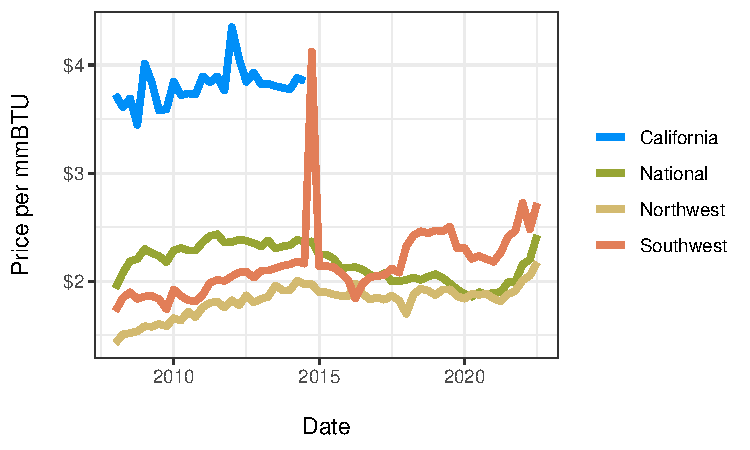
\includegraphics[width = 0.8\textwidth]{figures/chapter5_figures/coal_prices.pdf}
    \fignote[.8]{Figure displays the average price of coal sold to power plants in current dollars per million British Thermal Units (MMBtu) of states in each region. The series for California ends just before 2015 due to a declining number of coal plants and data confidentiality.}
\end{figure}

\begin{figure}
    \centering
    \caption{Natural Gas Prices by Region}
    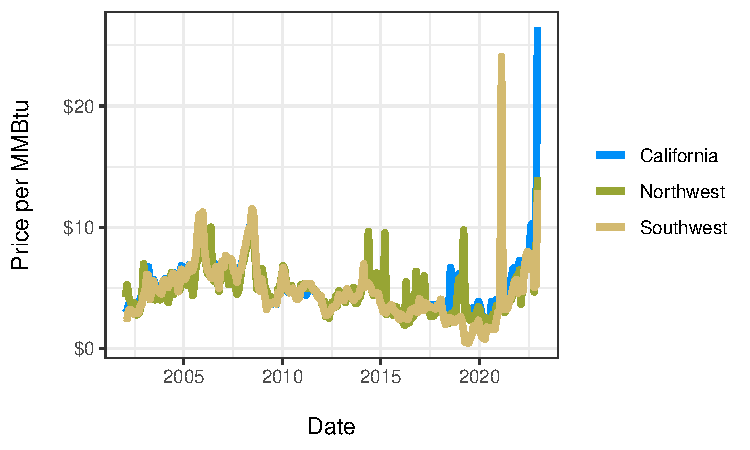
\includegraphics[width= 0.8\textwidth]{figures/chapter5_figures/gas_prices.pdf}
    \fignote[.8]{Figure displays the average price of natural gas sold to power plants in current dollars per million million British Thermal Units (MMBtu) of states in each region. Natural gas markets are generally more volatile than coal, and natural gas is usually more expensive than coal on a per MMBtu basis.}
\end{figure}

\begin{table}
    \centering
    \caption{Power Plant Summary Statistics}
\begin{tabular}{l c c c c c}
    \hline\hline
    Variable & Mean & St. Dev. & Min & Median & Max \\
    \hline\\[-1.8ex]
    \textit{Coal} \\
    \hline
    Capacity Factor & 0.524 & 0.188 & 0.135 & 0.526 & 0.892 \\ 
    Capacity (MW) & 730.438 & 691.725 & 1.500 & 525.900 & 2,441.900 \\ 
    Heat Rate (MMBtu/MWh) & 10.757 & 2.305 & 5.534 & 11.065 & 16.158 \\ 
    Input Price (\$/MWh) & 22.191 & 5.366 & 10.615 & 21.960 & 37.285 \\ 
    tonnes CO$_2$e/MWh & 1.042 & 0.226 & 0.527 & 1.075 & 1.580 \\ 
    kg NO$_x$/MWh & 0.859 & 0.462 & 0.210 & 0.826 & 2.344 \\ 
    kg SO$_2$/MWh & 1.056 & 2.113 & 0.001 & 0.436 & 10.109 \\ 
    kg PM2.5/MWh & 0.066 & 0.093 & 0.0001 & 0.039 & 0.522 \\ \\[-1.8ex]
    \textit{Gas} \\
    \hline
    Capacity Factor & 0.350 & 0.299 & 0.0004 & 0.297 & 0.972 \\ 
    Capacity (MW) & 197.335 & 314.527 & 0.900 & 49.800 & 1,857.000 \\ 
    Heat Rate (MMBtu/MWh) & 8.933 & 3.261 & 1.033 & 8.184 & 22.107 \\ 
    Input Price (\$/MWh) & 44.145 & 16.061 & 5.517 & 39.954 & 105.106 \\ 
    tonnes CO$_2$e/MWh & 0.475 & 0.178 & 0.000 & 0.434 & 1.342 \\ 
    kg NO$_x$/MWh & 1.410 & 3.323 & 0.000 & 0.154 & 24.725 \\ 
    kg SO$_2$/MWh & 0.014 & 0.090 & 0.000 & 0.003 & 1.253 \\ 
    kg PM2.5/MWh & 0.025 & 0.064 & 0.000 & 0.014 & 0.817 \\ \\[-1.8ex]
    \textit{Oil} \\
    \hline
    Capacity Factor & 0.175 & 0.280 & 0.0003 & 0.002 & 0.772 \\ 
    Capacity (MW) & 67.625 & 76.332 & 11.700 & 27.150 & 223.500 \\ 
    Heat Rate (MMBtu/MWh) & 19.456 & 13.205 & 8.015 & 17.343 & 48.441 \\ 
    Input Price (\$/MWh) & 223.093 & 151.417 & 91.903 & 198.863 & 555.443 \\ 
    tonnes CO$_2$e/MWh & 1.502 & 0.931 & 0.769 & 1.274 & 3.600 \\ 
    kg NO$_x$/MWh & 11.482 & 12.626 & 0.000 & 7.257 & 38.160 \\ 
    kg SO$_2$/MWh & 3.763 & 3.908 & 0.000 & 2.817 & 11.101 \\ 
    kg PM2.5/MWh & 0.723 & 1.277 & 0.023 & 0.121 & 3.682 \\ 
    \hline \\[-1.8ex] 
\end{tabular}
\fignote[1]{$N_\text{Coal} = 40$, $N_\text{Gas} = 433$, $N_\text{Oil} = 8$.}
\end{table}

\begin{figure}[!hbtp]
    \centering
    \caption{Nameplate Capacity Distribution by Generating Group \label{cluster_cap}}
    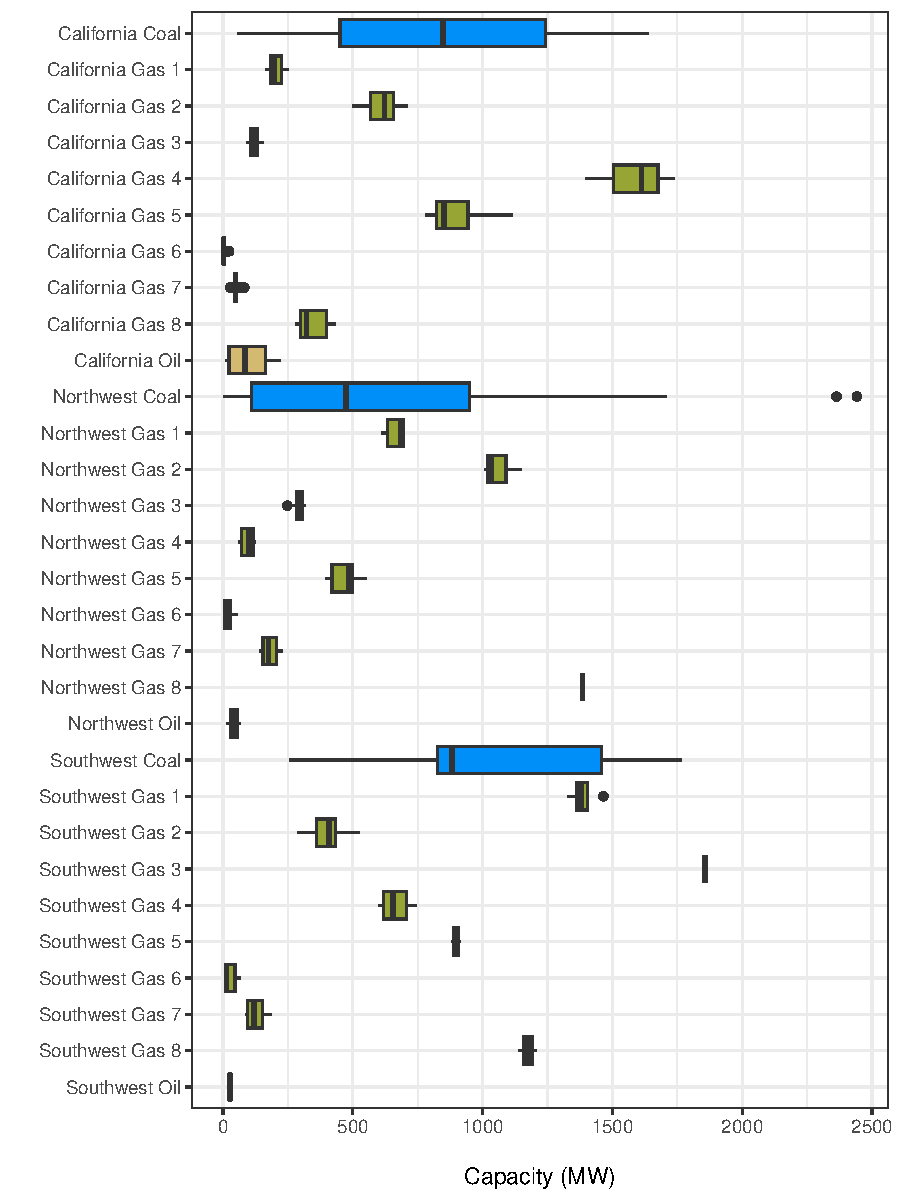
\includegraphics[width = 0.8\textwidth]{figures/chapter5_figures/kclusters_capacity.pdf}
    \fignote[.8]{Figure displays the distribution of the nameplate capacities of power plants in each of the thirty groups that emerges from the $k$-means clustering on set of power plants.}
\end{figure}

\begin{figure}[!hbtp]
    \centering
    \caption{Nameplate Capacity Distribution by Generating Group \label{cluster_hrate}}
    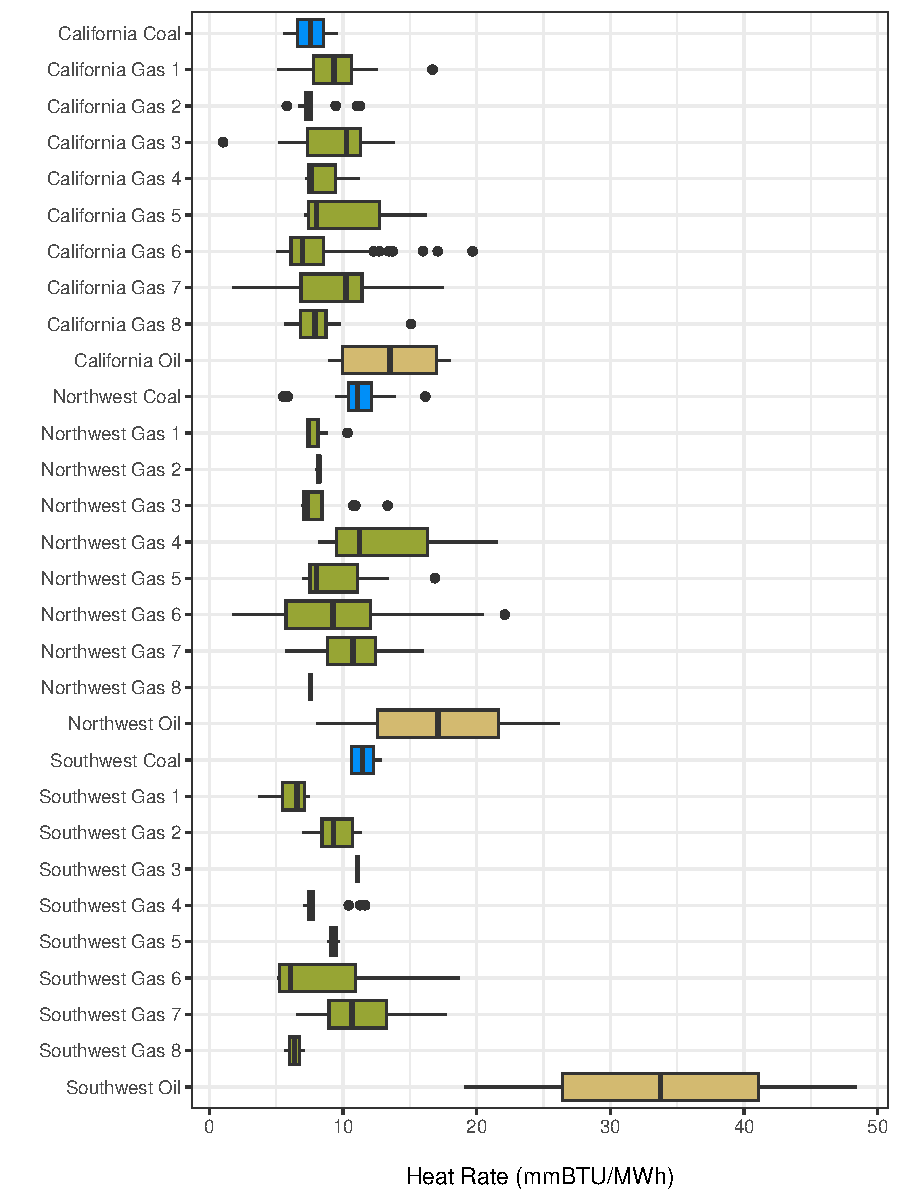
\includegraphics[width = 0.8\textwidth]{figures/chapter5_figures/kclusters_hrate.pdf}
    \fignote[.8]{Figure displays the distribution of the heat rates (MMBtu/Mwh) of power plants in each of the thirty groups that emerges from the $k$-means clustering on set of power plants.}
\end{figure}







\begin{figure}
    \centering
    \caption{Hourly Demand \label{hourly_demand}}
    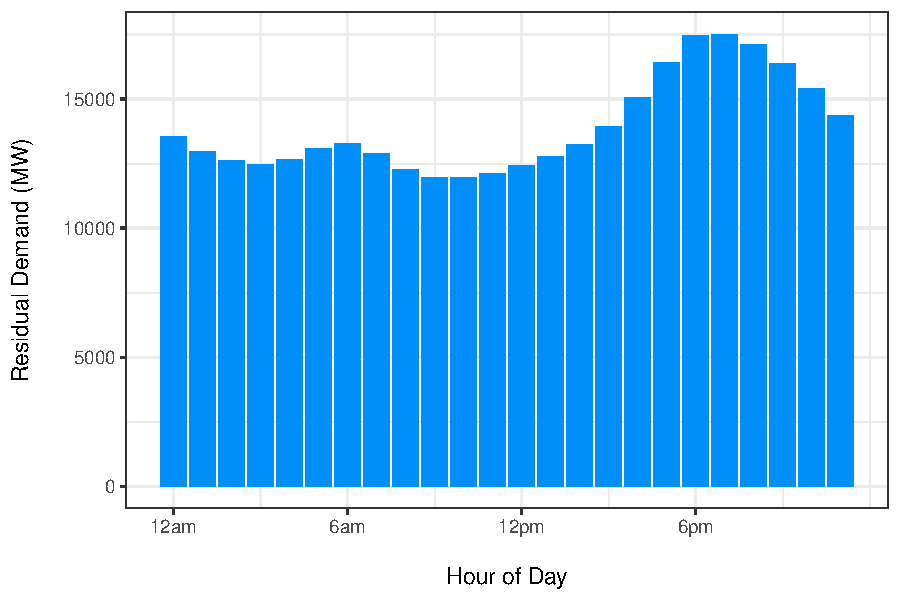
\includegraphics[width=0.7\textwidth]{figures/chapter5_figures/hourly_demand.pdf}
    \fignote[.9]{
        Figure shows the average hourly demand for electricity across he entire Western Interconnection. Demand usually dips to its loweest point around midmorning, and reaches its highest point in the evening.
    }
\end{figure}

\begin{figure}
    \centering
    \caption{Monthly Demand \label{monthly_demand}}
    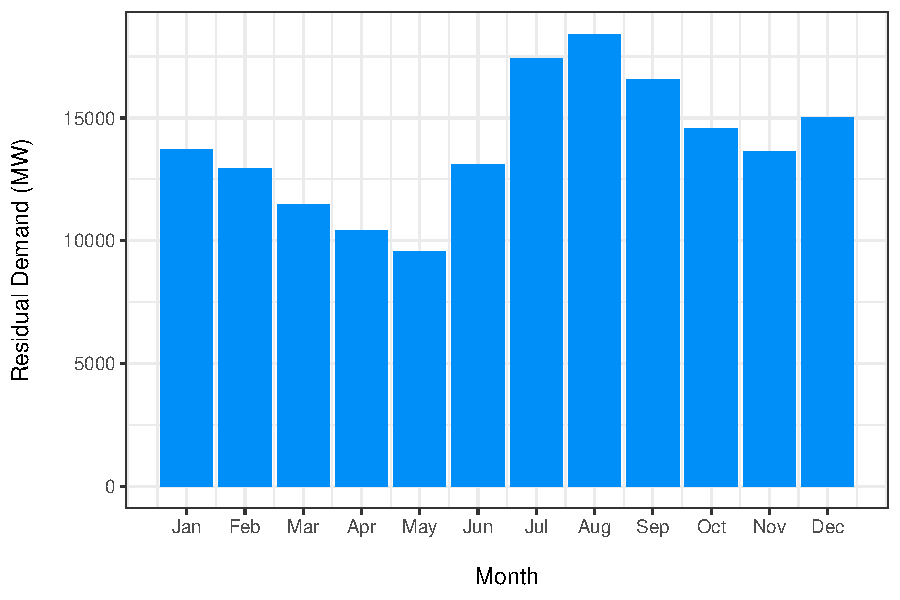
\includegraphics[width=0.7\textwidth]{figures/chapter5_figures/monthly_demand.pdf}
    \fignote[.9]{
        Figure shows the average monthly demand for electricity across he entire Western Interconnection. Demand usually dips to its loweest point around May, and reaches its highest point in the around August.
    }
\end{figure}

\newpage
\subsubsection*{Disadvantaged Communities \& Reconstructed EJ Index}

In this subsection I discuss the reconstruction of CalEnviroScreen 4.0 index for all Census tracts in the Western Interconnection. All data used to create the official CalEnviroScreen 4.0 index are available from the California Office of Environmental Health and Hazard Assessment (OEHHA). I begin by taking the raw data and using this to replicate the OEHHA's published index to ensure correct handling of missing data and correct weighting of individual components in the index. 

Each variable in the index belongs to one of four groups: Environmental Exposure Indicators, Environmental Effect Indicators, Sensitive Population Indicators, or Socioeconomic Factor Indicators. The EPA's Environmental Justice screening tool does not contain the exact same variables that go into the CalEnviroScreen index, but these are similar and fall into similar groups. Table \ref{DAC_crosswalk} displays the crosswalk between the variables in the original CalEnviroScreen index and the variables I use from the EPA's Environmental Justice screening tool to reconstruct the index.For each variable, I rank all Census tracts by their value for the variable and calculate the percentile each Census tract belongs to for each variable. Then for each of the four groups of variables, I average the Census tracts' percentile rankings for each the of the variables in the group. This average percentile forms a subindex for each of the four groups of the variables in the index. With these subindexes, I follow the CalEnviroScreen method for calculating the aggregated subindexes:
\begin{align*}
    \text{Pollution Burden} &= \tfrac23 \cdot \text{Envrionmental Exposure} + \tfrac13 \cdot \text{Environmental Effect}\\
    \text{Population Characteristics} &= \tfrac12 \cdot \text{Sensitive Population} + \tfrac12 \cdot \text{Socioeconomic Factor}
\end{align*}
Both of these aggregated subindexes, the Pollution Burden subindex and the Population Characteristics subindex, are then rescaled such that they are between 0 and 10 by finding the maximum value for each subindex, dividing all the scores by this value, and then multiplying by 10. Finally, the fully reconstructed index is the product of the rescaled Pollution Burden subindex and the rescaled Population Characteristics subindex. Rescaling the subindexes between 0 and 10 ensures that the full index is between 0 and 100. 

\begin{table}
    \centering
    \caption{Disadvantaged Community Index Comparison \label{DAC_crosswalk}}
    \small
    \begin{tabular}{L{0.2\textwidth} L{0.35\textwidth} L{0.35\textwidth}}
        \hline\hline \\ [-1.8ex]
        Index Category & CalEnviroScreen 4.0 Indicators & Replicated Indicators\\
        \hline
        Environmental Exposure Indicators & 
        \begin{itemize}[noitemsep, topsep=0pt]
            \item Air Quality: Ozone
            \item Air Quality: PM2.5
            \item Children's Lead Risk from Housing
            \item Diesel Particulate Matter
            \item Drinking Water Contaminants
            \item Pesticide Use
            \item Toxic Release from Facilities
            \item Traffic Impacts 
        \end{itemize} &
        \begin{itemize}[noitemsep, topsep=0pt]
            \item Ozone
            \item PM2.5
            \item Lead paint
            \item Diesel particulate matter
            \item Air toxics cancer risk
            \item Air toxics respiratory
            \item Traffic proximity
        \end{itemize} \\
        \hline
        Environmental Effect Indicators &
        \begin{itemize}[noitemsep, topsep=0pt]
            \item Cleanup Sites
            \item Groundwater Threats
            \item Hazardous Waste Generators \& Facilities
            \item Impaired Water Bodies
            \item Solid Waste Sites \& Facilities
        \end{itemize} &
        \begin{itemize}[noitemsep, topsep=0pt]
            \item Wastewater discharge
            \item Superfund proximity
            \item RMP facility proximity
            \item Hazardous waste proximity
            \item Underground storage tanks
        \end{itemize} \\
        \hline
        Sensitive Population Indicators & 
        \begin{itemize}[noitemsep, topsep=0pt]
            \item Asthma
            \item Cardiovascular Disease
            \item Low Birth Weight Infants
        \end{itemize} & 
        \begin{itemize}[noitemsep, topsep=0pt]
            \item \% under age 5
            \item \% over age 64
        \end{itemize} \\
        \hline 
        Socioeconomic Factor Indicators & 
        \begin{itemize}[noitemsep, topsep=0pt]
            \item Educational Attainment
            \item Housing Burden
            \item Linguistic Isolation
            \item Poverty
            \item Unemployment
        \end{itemize} & 
        \begin{itemize}[noitemsep, topsep=0pt]
            \item \% people of color
            \item \% low income
            \item \% less than high school education
            \item \% linguistically isolated
            \item Unemployment rate
            \item Demographic Index
        \end{itemize} \\
        \hline
    \end{tabular}
    \vspace{1em}
    \fignote[1]{
        Table displays the indicators in each of the four subindexes that make up the CalEnviroScreen 4.0 index compared to indicators used in to create the analogous index in the paper. 
    }
\end{table}

\begin{figure}
    \centering
    \caption{Disadvantaged Communities (DACs) Designation Comparison by Percentiles}
    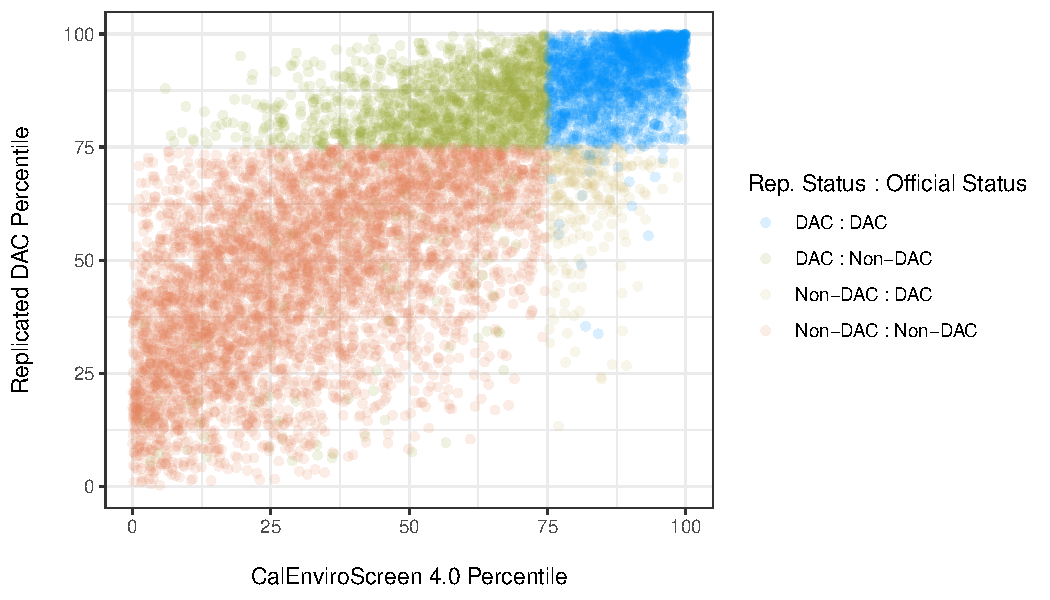
\includegraphics[width=1\textwidth]{figures/chapter5_figures/DAC_des_scatter.pdf}
    \fignote[1]{
        Figure displays the scatter plot between the percentile ranking of California Census tracts in CalEnviroScreen and the percentile rankings of California Census tracts in the reconstructed or replicated index. Blue dots indicate that a Census tract was identified as a DAC in both CalEnviroScreen and the reconstructed index, red dots indicate that a Census tract was identified as not a DAC in both CalEnviroScreen and the reconstructed index, green dots indicate that a Census tract was identified as a DAC in the reconstructed index but not the official index, and orange dots indicate that a Census tract was identified as a DAC in the official index but not the reconstructed index. There is a strong relationship between rankings in the orginal index and the replicated index.
    }
\end{figure}


\begin{table}[!htbp] \centering 
    \caption{Summary Statistics for Census Tracts in the Western Interconnection \label{dac_summary}} 
    \footnotesize
  \begin{tabular}{@{\extracolsep{3pt}}lcccccc} 
  \\[-1.8ex]\hline 
  \hline \\[-1.8ex] 
  & \multicolumn{3}{c}{Non-Disadvantaged} & \multicolumn{3}{c}{Disadvantaged} \\
    \cline{2-4} \cline{5-7}\\
  Statistic & Median & Mean & St. Dev. & Median & Mean & St. Dev.\\ 
  \hline \\ [-.8ex] 
    \emph{Pollution Burden} \\
    \hline \\[-.8ex]
    \%-ile Traffic proximity & 51.9 & 51.1 & 29.1 & 74.5 & 65.7 & 30.2 \\ 
    \%-ile Wastewater discharge & 54.9 & 53.5 & 31.6 & 77.4 & 66.9 & 30.3 \\  
    \%-ile Superfund proximity & 46.3 & 46.1 & 28.6 & 71.4 & 63.0 & 29.3 \\
    \%-ile Hazardous waste proximity & 60.9 & 55.8 & 29.1 & 86.4 & 74.7 & 28.5 \\ 
    \%-ile Ozone & 57.0 & 62.6 & 37.2  & 88.7 & 76.6 & 27.7 \\  
    \%-ile Particulate Matter 2.5 & 45.4 & 50.2 & 35.9  & 94.5 & 75.9 & 32.6 \\ \\[-.8ex]
    \emph{Population Characteristics} \\
    \hline \\[-.8ex]
    Total Population & 4,538 & 4,869.4 & 2,432.4 & 4,519 & 4,684.4 & 1,903.7 \\ 
    \% People of color & 33.2 & 37.7 & 23.2 & 80.6 & 72.5 & 24.7 \\  
    \% Low income & 22.9 & 25.6 & 15.0 & 44.4 & 44.1 & 16.9 \\ 
    \% Less than HS diploma & 6.9 & 9.3 & 8.6 & 23.6 & 25.2 & 14.4 \\ 
    \% Under age 5 & 5.4 & 5.5 & 2.6 & 7.0 & 7.1 & 2.6 \\ 
    \% Over age 64 & 14.7 & 16.4 & 9.8 & 12.1 & 13.4 & 7.3 \\ 
    Unemployment rate & 4.4 & 5.0 & 3.5 & 6.9 & 7.7 & 4.5 \\ 
  \hline \\[-1.8ex] 
  \end{tabular} 
  \fignote[1]{
    $N = 15,547$, $N_\text{Disadvantaged} = 4,587$, $N_\text{Non-disadvantaged} = 10,960$. Observations are 2010 Census tracts. All data on these Census tracts come from the EPA's Environmental Justice screening tool. 
  } 
\end{table} 

% High cost investment scenario
\begin{figure}
    \centering
    \caption{Power Plants Making Heat Rate Improving Investments---High Cost\label{hc_inv_region}}
    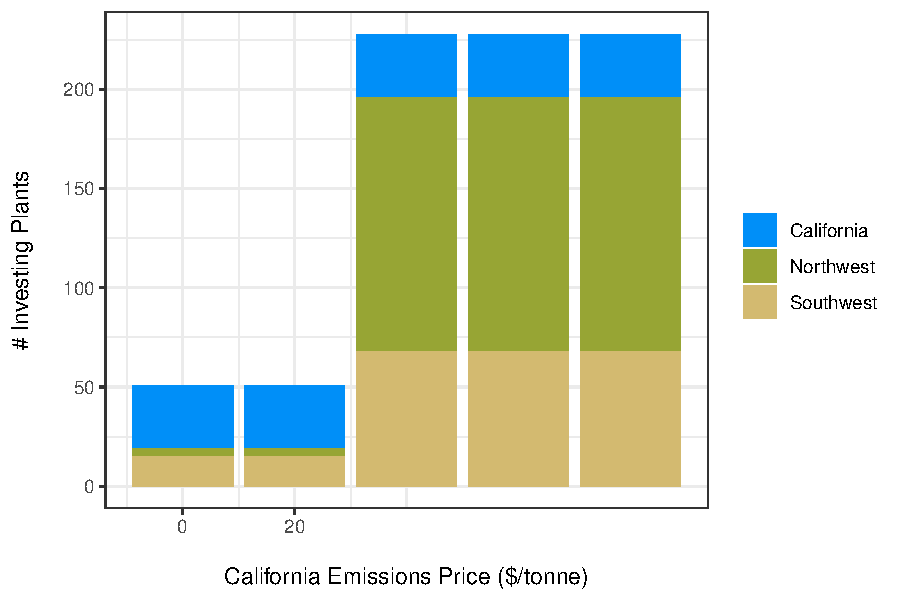
\includegraphics[width=0.8\textwidth]{figures/chapter5_figures/hc_inv_region.pdf}
    \fignote[.9]{
        Figure shows the number of power plants that make heat rate improving investments under each carbon price. These simulations all use a high investment cost scenario, where the investment costs for each power plant have been raised by a factor of ten. All policy scenarios in the figure include a BCA.
    }
\end{figure}

\begin{figure}
    \centering
    \caption{The EI Gap for SO$_2$ and PM2.5 in California \label{ei_gap_so2_pm25_cal}}
    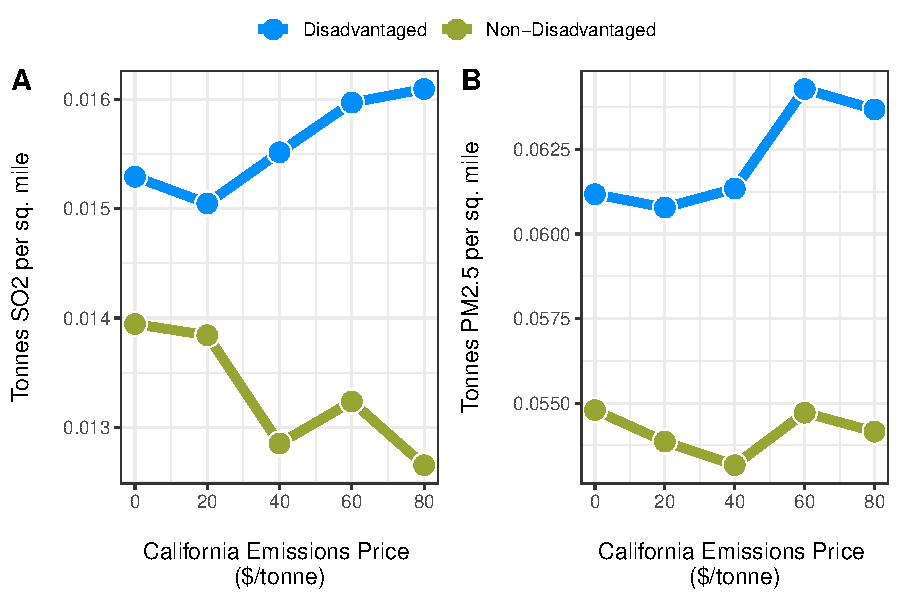
\includegraphics[width=\textwidth]{figures/chapter5_figures/ei_gap_so2_pm25_cal.pdf}
    \fignote[1]{
        Figure shows the simulated average concentration of SO$_2$ and PM2.5 for DACs and non-DACs across five different carbon prices for the subset of Census tracts in California. The distance between the two series is the EI Gap.
    }
\end{figure}
